%%%%%%%%%%%%%%%%%%%%%%%%%%%%%%%%%%%%%%%%%%%%%%%%%%%%%%%%%%%%%%%%%%%%%%%%%%%%%%%%%%
\begin{frame}[fragile]\frametitle{}
\begin{center}
{\Large Anova}
\end{center}
\end{frame}

%%%%%%%%%%%%%%%%%%%%%%%%%%%%%%%%%%%%%%%%%%%%%%%%%%%%%%%%%%%
\begin{frame}[fragile]\frametitle{Analysis of Variance (ANOVA)}
The difference between ANOVA and the t tests is that ANOVA can 
be  used  in  situations  where  there  are  two  or  more  means  being 
compared, whereas the t tests are limited to situations where only 
two means are involved. 
\end{frame}

%%%%%%%%%%%%%%%%%%%%%%%%%%%%%%%%%%%%%%%%%%%%%%%%%%%%%%%%%%%
\begin{frame}[fragile]\frametitle{Analysis of Variance (ANOVA)}
\begin{center}
\includegraphics[width=\linewidth,keepaspectratio]{anv1}
\end{center}
Finding DISTANCE between means

\tiny{(Reference: Statistics 101 - Brandon Foltz)}

\end{frame}

%%%%%%%%%%%%%%%%%%%%%%%%%%%%%%%%%%%%%%%%%%%%%%%%%%%%%%%%%%%
\begin{frame}[fragile]\frametitle{Analysis of Variance (ANOVA)}
Combine all data points from all 3 samples. Draw its distribution. Then compare of each with the combined one.
\begin{center}
\includegraphics[width=0.7\linewidth,keepaspectratio]{anv2}
\end{center}
$\bar{x}_1$ bang on combined mean, rest are a bit away.
\end{frame}

%%%%%%%%%%%%%%%%%%%%%%%%%%%%%%%%%%%%%%%%%%%%%%%%%%%%%%%%%%%
\begin{frame}[fragile]\frametitle{Analysis of Variance (ANOVA)}
New example: where $\bar{x}_3$  is far away. So not part of combined population. Outlier.

\begin{center}
\includegraphics[width=0.8\linewidth,keepaspectratio]{anv3}
\end{center}

\end{frame}

%%%%%%%%%%%%%%%%%%%%%%%%%%%%%%%%%%%%%%%%%%%%%%%%%%%%%%%%%%%
\begin{frame}[fragile]\frametitle{Analysis of Variance (ANOVA)}
New example: where both $\bar{x}_2$ and $\bar{x}_3$  are far away. All three are their OWN populations.

\begin{center}
\includegraphics[width=0.8\linewidth,keepaspectratio]{anv4}
\end{center}

\end{frame}

%%%%%%%%%%%%%%%%%%%%%%%%%%%%%%%%%%%%%%%%%%%%%%%%%%%%%%%%%%%
\begin{frame}[fragile]\frametitle{Analysis of Variance (ANOVA)}
\begin{center}
\includegraphics[width=0.8\linewidth,keepaspectratio]{anv5}
\end{center}
Variability is between means.
\end{frame}

%%%%%%%%%%%%%%%%%%%%%%%%%%%%%%%%%%%%%%%%%%%%%%%%%%%%%%%%%%%
\begin{frame}[fragile]\frametitle{Analysis of Variance (ANOVA)}
Pair wise t tests
\begin{center}
\includegraphics[width=0.8\linewidth,keepaspectratio]{anv6}
\end{center}
Combined error rate went from 5\% to 14.3\%. So we do not conduct multiple t tests.
\end{frame}

%%%%%%%%%%%%%%%%%%%%%%%%%%%%%%%%%%%%%%%%%%%%%%%%%%%%%%%%%%%
\begin{frame}[fragile]\frametitle{Analysis of Variance (ANOVA)}
Each distribution has its own internal variance / variability. Anova is a variability ratio.
\begin{center}
\includegraphics[width=0.8\linewidth,keepaspectratio]{anv7}
\end{center}
\end{frame}

%%%%%%%%%%%%%%%%%%%%%%%%%%%%%%%%%%%%%%%%%%%%%%%%%%%%%%%%%%%
\begin{frame}[fragile]\frametitle{Analysis of Variance (ANOVA)}
Total variance has two components.
\begin{center}
\includegraphics[width=0.8\linewidth,keepaspectratio]{anv8}
\end{center}
\end{frame}

%%%%%%%%%%%%%%%%%%%%%%%%%%%%%%%%%%%%%%%%%%%%%%%%%%%%%%%%%%%
\begin{frame}[fragile]\frametitle{Analysis of Variance (ANOVA)}
\begin{center}
\includegraphics[width=0.8\linewidth,keepaspectratio]{anv9}
\end{center}
\end{frame}

%%%%%%%%%%%%%%%%%%%%%%%%%%%%%%%%%%%%%%%%%%%%%%%%%%%%%%%%%%
\begin{frame}[fragile]\frametitle{Analysis of Variance (ANOVA)}
\begin{center}
\includegraphics[width=0.8\linewidth,keepaspectratio]{anv11}
\end{center}
\end{frame}

%%%%%%%%%%%%%%%%%%%%%%%%%%%%%%%%%%%%%%%%%%%%%%%%%%%%%%%%%%%
\begin{frame}[fragile]\frametitle{Analysis of Variance (ANOVA)}
\begin{center}
\includegraphics[width=0.8\linewidth,keepaspectratio]{anv10}
\end{center}
\end{frame}

%  https://www.youtube.com/watch?v=JgMFhKi6f6Y

%
%
%%%%%%%%%%%%%%%%%%%%%%%%%%%%%%%%%%%%%%%%%%%%%%%%%%%%%%%%%%%
%\begin{frame}[fragile]\frametitle{Analysis of Variance (ANOVA)}
%SS is variance without averaging
%\begin{center}
%\includegraphics[width=0.8\linewidth,keepaspectratio]{anv12}
%\end{center}
%\end{frame}
%
%%%%%%%%%%%%%%%%%%%%%%%%%%%%%%%%%%%%%%%%%%%%%%%%%%%%%%%%%%%
%\begin{frame}[fragile]\frametitle{Analysis of Variance (ANOVA)}
%Total SS = SSC (variance between) + SSE (variance within)
%\begin{center}
%\includegraphics[width=0.8\linewidth,keepaspectratio]{anv13}
%\end{center}
%\end{frame}
%
%%%%%%%%%%%%%%%%%%%%%%%%%%%%%%%%%%%%%%%%%%%%%%%%%%%%%%%%%%%
%\begin{frame}[fragile]\frametitle{Analysis of Variance (ANOVA)}
%21 SS make up SST
%\begin{center}
%\includegraphics[width=0.8\linewidth,keepaspectratio]{anv14}
%\end{center}
%\end{frame}
%
%
%
%%%%%%%%%%%%%%%%%%%%%%%%%%%%%%%%%%%%%%%%%%%%%%%%%%%%%%%%%%%
%\begin{frame}[fragile]\frametitle{Analysis of Variance (ANOVA)}
%\begin{itemize}
%\item Analysis  of  variance  is  necessary  to  protect  researchers  from 
%excessive  risk  of  a  Type  I  error  in  situations  where  a  study  is 
%comparing more than two population means.   
%\item These situations would require a series of several t tests to evaluate 
%all of the mean differences.  (Remember, a t test can compare only 
%2 means at a time.)   
%\end{itemize}
%\end{frame}
%
%%%%%%%%%%%%%%%%%%%%%%%%%%%%%%%%%%%%%%%%%%%%%%%%%%%%%%%%%%%%
%\begin{frame}[fragile]\frametitle{Analysis of Variance (ANOVA)}
%\begin{itemize}
%\item ANOVA allows researcher to evaluate all of the mean differences 
%in  a  single  hypothesis  test  using  a  single  $\alpha$-level  and,  thereby, 
%keeps the risk of a Type I error under control no matter how many 
%different means are being compared. 
%\item Although  ANOVA  can  be  used  in  a  variety  of  different  research 
%situations,  this  chapter  presents  only  independent-measures 
%designs involving only one independent variable.  
%\end{itemize}
%\end{frame}
%
%%%%%%%%%%%%%%%%%%%%%%%%%%%%%%%%%%%%%%%%%%%%%%%%%%%%%%%%%%%
%\begin{frame}[fragile]\frametitle{Analysis of Variance (ANOVA)}
%\begin{center}
%\includegraphics[width=\linewidth,keepaspectratio]{anova1}
%\end{center}
%\end{frame}
%
%
%%%%%%%%%%%%%%%%%%%%%%%%%%%%%%%%%%%%%%%%%%%%%%%%%%%%%%%%%%%
%\begin{frame}[fragile]\frametitle{Analysis of Variance (ANOVA)}
%\begin{itemize}
%\item The  null  hypothesis  for  ANOVA  states  that  for  the  general  population 
%there are no mean differences among the treatments being compared
%\item When  the  null  hypothesis  is  rejected,  the  conclusion  is  that  there  are 
%significant mean differences.  
%\end{itemize}
%\end{frame}
%
%%%%%%%%%%%%%%%%%%%%%%%%%%%%%%%%%%%%%%%%%%%%%%%%%%%%%%%%%%%
%\begin{frame}[fragile]\frametitle{Analysis of Variance (ANOVA)}
%\begin{itemize}
%\item However,  the  ANOVA  simply  establishes  that  differences  exist,  it  does 
%not indicate exactly which treatments are different.   
%\item For testing which treatments are significantly different from each other, 
%we can use multiple comparison tests. 
%\end{itemize}
%\end{frame}
%
%%%%%%%%%%%%%%%%%%%%%%%%%%%%%%%%%%%%%%%%%%%%%%%%%%%%%%%%%%%
%\begin{frame}[fragile]\frametitle{Analysis of Variance (ANOVA)}
%\begin{itemize}
%\item The test statistic for ANOVA is an F-ratio, which is a ratio of two sample 
%variances.    In  the  context  of  ANOVA,  the  sample  variances  are  called 
%mean squares, or MS values.   
%\item The  top  of  the  F-ratio  $MS_{between}$
%  measures  the  size  of  mean  differences 
%between  samples.    The  bottom  of  the  ratio  $MS_{within}$
%  measures  the 
%magnitude of differences that would be expected without any treatment 
%effects.  
%\end{itemize}
%\end{frame}
%
%%%%%%%%%%%%%%%%%%%%%%%%%%%%%%%%%%%%%%%%%%%%%%%%%%%%%%%%%%%
%\begin{frame}[fragile]\frametitle{Analysis of Variance (ANOVA)}
%Thus, the F-ratio has the same basic structure as the independent-
%measures t statistic. 
%\begin{center}
%\includegraphics[width=0.5\linewidth,keepaspectratio]{anova2}
%\end{center}
%\end{frame}
%
%%%%%%%%%%%%%%%%%%%%%%%%%%%%%%%%%%%%%%%%%%%%%%%%%%%%%%%%%%%%
%\begin{frame}[fragile]\frametitle{Analysis of Variance (ANOVA)}
%\begin{itemize}
%\item A  large  value  for  the  F-ratio  indicates  that  the  obtained  sample 
%mean  differences  are  greater  than  would  be  expected  if  the 
%treatments had no effect. 
%\item Each  of  the  sample  variances,  MS  values,  in  the  F-ratio  is 
%computed using the basic formula for sample variance: $$ MS = \frac{SS}{df}$$
%\end{itemize}
%\end{frame}
%
%%%%%%%%%%%%%%%%%%%%%%%%%%%%%%%%%%%%%%%%%%%%%%%%%%%%%%%%%%%%
%\begin{frame}[fragile]\frametitle{Analysis of Variance (ANOVA)}
%To obtain the SS and df values, you must go through an analysis 
%that separates the total variability for the entire set of data into two 
%basic  components:  between-treatment  variability  (which  will 
%become  the  numerator  of  the  F-ratio),  and  within-treatment 
%variability (which will be the denominator).  
%
%\end{frame}
%
%%%%%%%%%%%%%%%%%%%%%%%%%%%%%%%%%%%%%%%%%%%%%%%%%%%%%%%%%%%%
%\begin{frame}[fragile]\frametitle{Analysis of Variance (ANOVA)}
%Considering these sources of variability, the structure of the F-ratio 
%becomes, 
%\begin{center}
%\includegraphics[width=0.5\linewidth,keepaspectratio]{anova3}
%\end{center}
%\end{frame}
%
%%%%%%%%%%%%%%%%%%%%%%%%%%%%%%%%%%%%%%%%%%%%%%%%%%%%%%%%%%
%\begin{frame}[fragile]\frametitle{Analysis of Variance (ANOVA)}
%\begin{itemize}
%\item When  the  null  hypothesis  is  true  and  there  are  no  differences 
%between treatments, the F-ratio is balanced.   
%\item That is, when the "treatment effect" is zero, the top and bottom of 
%the F-ratio are measuring the same variance.   
%\item In  this  case,  you  should  expect  an  F-ratio  near  1.00.    When  the 
%sample  data  produce  an  F-ratio  near  1.00,  we  will  conclude  that 
%there is no significant treatment effect. 
%\end{itemize}
%\end{frame}
%%%%%%%%%%%%%%%%%%%%%%%%%%%%%%%%%%%%%%%%%%%%%%%%%%%%%%%%%%%%
%\begin{frame}[fragile]\frametitle{Analysis of Variance (ANOVA)}
%\begin{itemize}
%\item On  the  other  hand,  a  large  treatment  effect  will  produce  a  large 
%value for the F-ratio.  Thus, when the sample data produce a large 
%\item F-ratio we will reject the null hypothesis and conclude that there 
%are significant differences between treatments. 
%\item To determine whether an F-ratio is large enough to be significant, 
%you must select an $\alpha$-level, find the df values for the numerator and 
%denominator of the F-ratio, and consult the F-distribution table to 
%find the critical value.  
%\end{itemize}
%\end{frame}


%%%%%%%%%%%%%%%%%%%%%%%%%%%%%%%%%%%%%%%%%%%%%%%%%%%%
%\begin{frame}[fragile]\frametitle{T-Test}
%The two normal probability distribution functions (p.d.f) stacked on top of each other look like this:
%\begin{center}
%\includegraphics[width=\linewidth,keepaspectratio]{ttest1}
%\end{center}
%\end{frame}
%
%%%%%%%%%%%%%%%%%%%%%%%%%%%%%%%%%%%%%%%%%%%%%%%%%%%%
%\begin{frame}[fragile]\frametitle{T-Test}
%One sample T test: sample mean is equial to population mean $m = \mu$
%\begin{lstlisting}
%true_mu = 0
%
%onesample_results = scipy.stats.ttest_1samp(data1, true_mu)
%
%matrix_onesample = [
%    ['', 'Test Statistic', 'p-value'],
%    ['Sample Data', onesample_results[0], onesample_results[1]]
%]
%
%onesample_table = FF.create_table(matrix_onesample, index=True)
%py.iplot(onesample_table, filename='onesample-table')
%\end{lstlisting}
%\end{frame}
%
%


%
%\begin{frame}
%\frametitle{Two-sample comparisons}
%
%Suppose we are comparing samples from two populations, and we are
%interested in whether the two population means are equal.
%
%This is a very common setting.  Here are two specific examples:
%
%\begin{itemize}
%
%\item We are interested in comparing two treatments for high blood
%  pressure.  Each treatment lowers blood pressure on average by a
%  certain amount.  We would like to know the difference between the
%  two population ``treatment effects.''
%
%\item Visitors to a web site are shown one of two different
%  advertisements for the same product.  We are able to obtain the
%  fraction of the time that the user clicks on the ad (the ``click
%  rate'').  We would like to know the population value of the
%  difference in click rates.
%
%\end{itemize}
%
%\end{frame}
%
%\begin{frame}
%\frametitle{Two-sample comparisons}
%
%\begin{center}
%\scalebox{0.9}{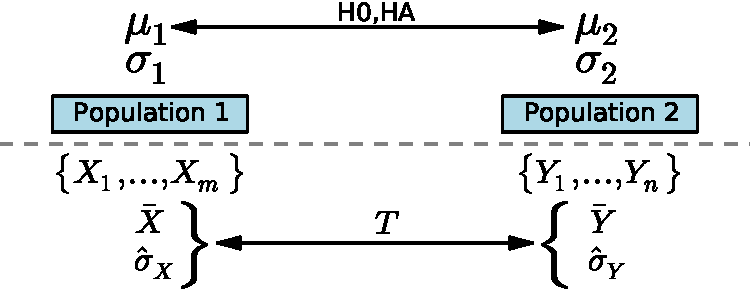
\includegraphics{015.pdf}}
%\end{center}
%
%\end{frame}
%
%\begin{frame}
%\frametitle{Two-sample comparisons}
%
%Let $X_1, \ldots, X_n$ denote the data from the first population, and
%$Y_1, \ldots, Y_m$ denote the data from the second population.  Let
%$\bar{X}$ and $\bar{Y}$ denote the two sample means.
%
%We can estimate the difference in population means using
%$\bar{X}-\bar{Y}$.  If the population means are $\mu_X$ and $\mu_Y$,
%then $\bar{X}-\bar{Y}$ is an unbiased estimate of the mean difference
%$\mu_X-\mu_Y$, i.e.
%
%$$ E(\bar{X}-\bar{Y}) = \mu_X - \mu_Y.
%$$
%
%\end{frame}
%
%
%\begin{frame}
%\frametitle{Two-sample comparisons}
%
%For testing, we can consider the \textcolor{purple}{null hypothesis}
%$\mu_X = \mu_Y$.
%
%As a test statistic, we can start with $D = \bar{X} - \bar{Y}$, but we
%will need to standardize it.
%
%Under the null hypothesis, $ED = 0$.  The variance of $D$ is 
%
%\begin{eqnarray*}
%{\rm var}(\bar{X} - \bar{Y}) &=& {\rm var}(\bar{X}) + {\rm
%  var}(-\bar{Y})\\ &=& {\rm var}(\bar{X}) + {\rm
%  var}(\bar{Y})\\ &=& \sigma_X^2/n + \sigma_Y^2/m.
%\end{eqnarray*}
%
%Thus the {\bf two-sample Z-statistic}
%
%$$
%T \equiv \frac{\bar{X} - \bar{Y}}{\sqrt{\sigma_X^2/n + \sigma_Y^2/m}}
%$$
%
%has a standardized distribution under the null
%hypothesis.
%
%\end{frame}
%
%
%\begin{frame}
%\frametitle{Two-sample comparisons}
%
%A test statistic value of $T=0$ is perfectly consistent with the null
%hypothesis.  Larger values of $|T|$ indicate increasing levels of
%evidence against the null hypothesis.
%
%The \textcolor{purple}{p-value} is the null distribution probability
%that as much evidence or more evidence against the null is observed
%(hypothetically, if the null hypothesis were true) than was actually
%observed:
%
%$$
%p = P_0(|T| \ge |T_{\rm obs}|)
%$$
%
%This is the {\bf 2-sided p-value} -- there are similar expressions for
%one-sided (right and left tail) p-values.
%
%\end{frame}
%
%
%\begin{frame}
%\frametitle{Two-sample comparisons}
%
%Treating the test statistic $T$ as having a standard normal
%distribution under the null hypothesis, the p-value can be computed as
%
%\begin{eqnarray*}
%P_0(|T| \ge |T_{\rm obs}|) &=& P_0(T \ge |T_{\rm obs}|) + P_0(T \le
%-|T_{\rm obs}|)\\ &=& 2\cdot P(T \le -|T_{\rm obs}|),
%\end{eqnarray*}
%
%where $P_0(T \ge |T_{\rm obs}|) = P_0(T \le -|T_{\rm obs}|)$ due to the
%symmetry of the normal distribution.
%
%\end{frame}
%
%
%\begin{frame}
%\frametitle{Acceptance/rejection of hypotheses}
%
%An alternative framework (to p-values) for hypothesis testing is based
%on the idea that a null hypothesis is \textcolor{purple}{rejected} if
%$|T|$ is sufficiently large, and otherwise is
%\textcolor{purple}{accepted}.  
%
%In this setting, there are two ways we can make the correct decision
%and two ways we can make the wrong decision:
%
%\bigskip
%
%\begin{center}
%\begin{tabular}{lll}
%              & Accept $H_0$ & Reject $H_0$\\\hline
%$H_0$ is true & Correct      & Type I error\\
%$H_A$ is true & Type II error & Correct\\\hline
%\end{tabular}
%\end{center}
%
%\bigskip
%
%The \textcolor{purple}{level} of a hypothesis test is the probability
%that a type I error occurs.
%
%\end{frame}
%
%\begin{frame}
%\frametitle{Acceptance/rejection of hypotheses}
%
%Suppose the sampling distribution of $T$ under the null hypothesis is
%standard normal and we reject the null hypothesis when $|T|>2$.
%
%There are two ways we can reject -- either when $T>2$ or when $T<-2$.
%Each of these events has probability 0.025, so the type I error is
%0.05.
%
%\bigskip
%
%\begin{center}
%\scalebox{0.6}{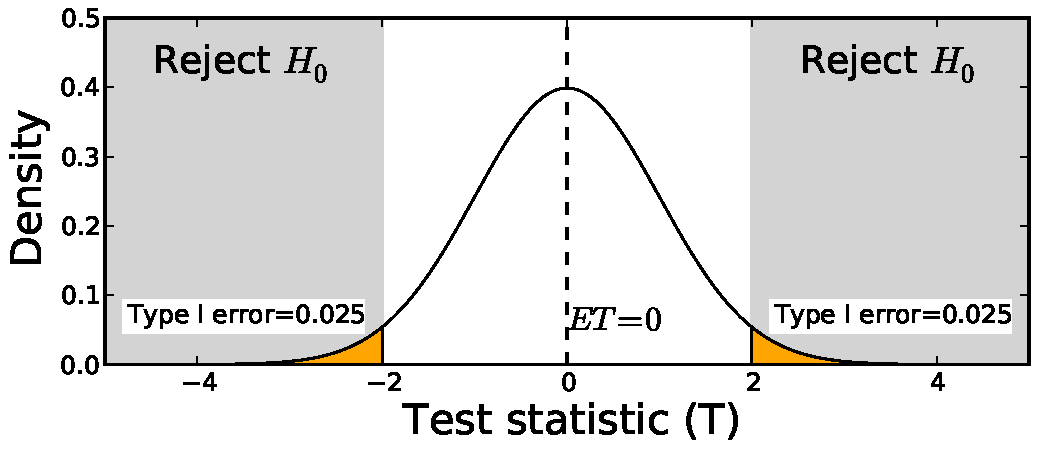
\includegraphics{049.pdf}}
%\end{center}
%
%
%\end{frame}
%
%
%\begin{frame}
%\frametitle{Two-sample tests with unknown variances}
%
%If the variances in the $X$ and $Y$ populations are unknown, we can
%use the estimated variance
%
%$$
%\hat{\sigma}_X^2/n + \hat{\sigma}_Y^2/m.
%$$
%
%In this case the test statistic is approximately t-distributed with
%the following degrees of freedom:
%
%$$ \frac{(\sigma_X^2/n + \sigma_Y^2/m)^2}{(\sigma_X^2/n)^2/(n-1) +
%(\sigma_Y^2/m)^2/(m-1)}.
%$$
%
%\end{frame}
%
%
%\begin{frame}
%\frametitle{Power of hypothesis tests}
%
%\begin{center}
%The \textcolor{purple}{power} of a hypothesis test is the probability
%of rejecting the null hypothesis when the alternative hypothesis is
%true.
%
%\end{center}
%
%Here are two equivalent ways of describing the power:
%
%\begin{itemize}
%
%\item The power is the probability of getting a p-value below a
%  defined value (usually 0.05) when the alternative hypothesis is
%  true.
%
%\item If the test statistic $T$ is standardized under the null
%  hypothesis, the power is the probability that $T$ exceeds the
%  critical value (usually $2$) when the alternative hypothesis is true.
%
%\end{itemize}
%
%The power depends on the sample size and the \textcolor{purple}{effect
%  size}, which is a measure of how distinguishable the null and
%alternative hypotheses are from each other.
%
%\end{frame}
%
%\begin{frame}
%\frametitle{Power of two-sample hypothesis tests}
%
%The effect size is related to two other quantities:
%
%\begin{itemize}
%
%\item The \textcolor{purple}{raw (unstandardized) effect size} is the
%  difference in population means of the two groups being compared.
%
%\item The \textcolor{purple}{response variability} is a summary of the
%  differences among individuals that are not related to their
%  treatment status.
%
%\end{itemize}
%
%Power is positively related to the raw effect size and is inversely
%related to response variability.
%
%\textcolor{blue}{\bf Example:} We have more power to detect a given
%treatment effect if everyone's blood pressure drops by 5 units, than
%if half of the subjects have a 10 unit decline and half of the
%subjects have no decline at all (even though the average decline is 5
%units in both cases).
%
%\end{frame}
%
%\begin{frame}
%\frametitle{Power of two-sample hypothesis tests}
%
%The two-sample Z-test statistic can be rewritten as
%
%$$
%T = \sqrt{m+n}\frac{\bar{X} - \bar{Y}}{\sqrt{\sigma_X^2/q_X + \sigma_Y^2/q_Y}},
%$$
%
%where $q_X = n/(n+m)$ and $q_Y = m/(n+m)$ are the proportions of the
%overall sample drawn from each of the two populations.
%
%Most test statistics can be written in this form
%
%$$ \sqrt{\rm total\;sample\;size}\times{\rm a\;``stable\;value''}
%$$
%
%Here the total sample size is $m+n$ and the ``stable
%value'' is
%
%$$
%\frac{\bar{X} - \bar{Y}}{\sqrt{\sigma_X^2/q_X + \sigma_Y^2/q_Y}}.
%$$
%
%\end{frame}
%
%\begin{frame}
%\frametitle{Power of two-sample hypothesis tests}
%
%By the central limit theorem, we know that under the null hypothesis,
%as $m$ and $n$ grow, $T$ becomes increasingly well approximated by a
%standard normal distribution.
%
%Under the alternative hypothesis, we have
%
%$$ E\frac{\bar{X} - \bar{Y}}{\sqrt{\sigma_X^2/q_X + \sigma_Y^2/q_Y}} =
%\frac{\mu_X - \mu_Y}{\sqrt{\sigma_X^2/q_X + \sigma_Y^2/q_Y}} \equiv
%\Delta.
%$$
%
%Thus the expected test statistic is approximately equal to
%$\sqrt{m+n}\cdot\Delta$ -- it continues to grow (at ``rate''
%$\sqrt{m+n}$) as the sample size grows.
%
%\end{frame}
%
%
%\begin{frame}
%\frametitle{Power of two-sample hypothesis tests}
%
%Here we see the density function of the test statistic, in a case
%where its expected value is $ET=2.5$:
%
%\begin{center}
%\scalebox{0.6}{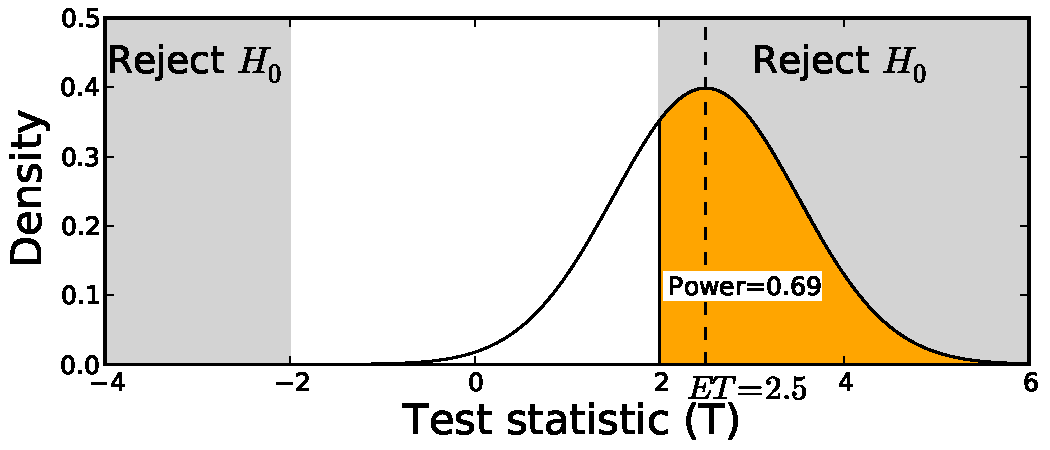
\includegraphics{047.pdf}}
%\end{center}
%
%If the test statistic falls in the grey region, we reject the null
%hypothesis.  The power is the probability of this happening, indicated
%by the orange region.
%
%Note that the standard deviation of the test statistics is one.
%
%\end{frame}
%
%
%\begin{frame}
%\frametitle{Power of two-sample hypothesis tests}
%
%For the two-sample problem, we can use $\delta = \mu_X - \mu_Y$ as the
%raw (unstandardized) effect size.
%
%The power is
%
%$$
%P(|T| \ge 2) = P(T \ge 2) + P(T \le -2).
%$$
%
%The first summand is
%
%\begin{eqnarray*}
%P(T\ge 2) &=& P\left(\sqrt{m+n}\frac{\bar{X} -
%  \bar{Y}}{\sqrt{\sigma_X^2/q_X + \sigma_Y^2/q_Y}} \ge 2\right)\\ &=&
%P\left(\sqrt{m+n}\frac{\bar{X} - \bar{Y} -
%  \delta}{\sqrt{\sigma_X^2/q_X + \sigma_Y^2/q_Y}}
%\ge\right.\\&&\;\;\;\;\;\; \left. 2 -
%\delta\sqrt{(m+n)/(\sigma_X^2/q_X + \sigma_Y^2/q_Y)}\right).
%\end{eqnarray*}
%
%\end{frame}
%
%
%\begin{frame}
%\frametitle{Power of two-sample hypothesis tests}
%
%Under the alternative hypothesis, $\bar{X} - \bar{Y} - \delta$ has
%mean zero, so 
%
%$$ \sqrt{m+n}\frac{\bar{X} - \bar{Y} - \delta}{\sqrt{\sigma_X^2/q_X +
%\sigma_Y^2/q_Y}}
%$$
%
%can be treated as being standard normal.  Thus
%
%$$ P(T> 2) = 1 - P\left(Z \le 2 - \delta\sqrt{(m+n)/(\sigma_X^2/q_X +
%\sigma_Y^2/q_Y)}\right),
%$$
%
%which can be obtained from a standard normal probability table.
%
%A similar calculation can be used to get an expression for $P(T \le
%-2)$.
%
%Note that as $\delta$ grows and/or $m+n$ grows and/or $\sigma_X$ and
%$\sigma_Y$ shrink, the power gets closer and closer to 1.
%
%\end{frame}
%
%
%\begin{frame}
%\frametitle{Power (determining sample size)}
%
%We often need to assess what sample size would be required to detect
%an effect in a particular situation.
%
%For example, we may be interested in detecting a treatment effect in
%which a drug lowers a particular quantity by two units on average.  We
%may be also be willing to assume (for the purposes of power analysis)
%that this quantity varies with a standard deviation of 3 units (for
%both treated and untreated subjects). Suppose also
%that we intend to carry out our study using equal numbers of treated
%and untreated subjects.
%
%In the notation of the preceding slides, we have
%
%\begin{itemize}
%
%\item $\mu_X-\mu_Y = 2$ (This is the raw, or unstandardized treatment
%  effect, where X is the untreated group and Y is the treated group.)
%
%\item $\sigma_X = \sigma_Y = 3$ (This is the variability of
%  individual subjects' blood pressures around the mean of the group
%  they belong to (either treated or untreated.)
%
%\item $q_X = q_Y = 1/2$ (This is our ``design decision'' to use
%  equal numbers of treated and untreated subjects.)
%
%\end{itemize}
%
%\end{frame}
%
%
%\begin{frame}
%\frametitle{Power (determining sample size)}
%
%So the ``stable value'' $\Delta$ is
%
%$$
%\Delta = \frac{2}{\sqrt{9/(1/2) + 9/(1/2)}} = 1/3
%$$
%
%Thus the test-statistic will have mean value equal to
%
%\begin{center}
%$\sqrt{m+n}\cdot\Delta = \sqrt{2n}/3$
%\end{center}
%
%To reject the null hypothesis at the usual (two-sided $\alpha=0.05$)
%level, we need the test statistic to be greater than 2.  Thus we have
%$\sqrt{2n}/3>2$, or $n>18$ to get 50\% power.
%
%If we want 80\% power, then we need to solve
%
%\vspace{-0.5cm}
%
%$$
%0.8 = P(T>2) = P(T-ET>2-ET) = P(Z>2-\sqrt{2n}/3).
%$$
%
%Since the 20${\rm th}$ percentile of a standard normal distribution is
%$-0.84$, this gives us $2-\sqrt{2n}/3 = -0.84$, so we
%need $n=36$ to get 80\% power.
%
%\end{frame}
%
%
%\begin{frame}
%\frametitle{Power (determining effect size)}
%
%A different type of power analysis comes up when the sample size is
%fixed, and we are asked to determine what effects can be detected at
%that sample size.
%
%Suppose we are given that a comparison of two treatments will involve
%20 treated subjects, and 40 untreated subjects, and we are willing to
%assume (for the purposes of power analysis), that the standard
%deviation within the treated subjects is 1 and the standard deviation
%within the untreated subjects is 2.
%
%We have
%
%\begin{itemize}
%
%\item $\sigma_X = 1$, $\sigma_Y = 2$
%
%\item $q_X = 1/3$, $q_Y = 2/3$
%
%\item $\sqrt{m+n} = \sqrt{60} \approx 7.75$.
%
%\end{itemize}
%
%We now need to determine what values of $\delta = \mu_x-\mu_y$ would
%allow us to reject the null hypothesis with reasonably high frequency.
%
%\end{frame}
%
%
%\begin{frame}
%\frametitle{Power (determining effect size)}
%
%The expected value of the test statistic is
%
%$$ \sqrt{m+n}\cdot\Delta \approx
%7.75\cdot\frac{\mu_x-\mu_y}{\sqrt{1/(1/3) + 2/(2/3)}} \approx
%2.6\delta.
%$$
%
%To get 80\% power, we need
%
%$$
%0.8 = P(T>2) = P(T-ET>2-ET) = P(Z>2-2.6\delta).
%$$
%
%Thus we have $2-2.6\delta = -0.84$, so $\delta = 1.09$ is
%required.
%
%\end{frame}
%
